
\begin{minipage}{11cm}
\section{Adaptive Signalverarbeitung}
\subsection{Adaptive Filter}
\textbf{Ziel:} Verarbeitungseigenschaften des adaptiven Systems selbstst�ndig durch rekursive Modifikation seiner Parameter $c_n$ �ndern.

\subsubsection{LS (Least Square) Algorithmus - Wiener L�sung}

\end{minipage}
\begin{minipage}{8cm}
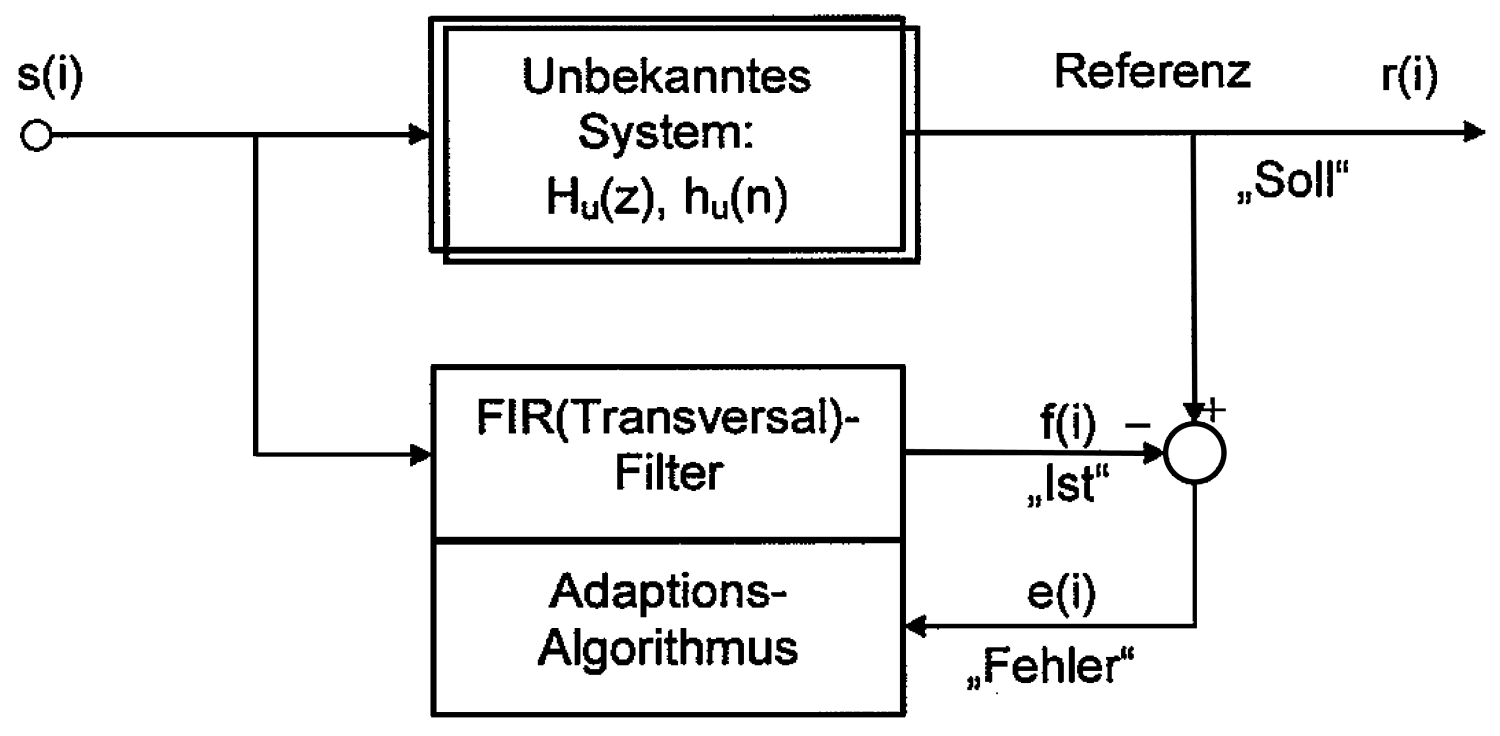
\includegraphics[width=8cm,trim= 0cm 0cm 0cm 0cm]{Content/AdaptSigVer/AdaptSigVer.png}
\end{minipage}

F�r Berechnung der AKF $Rss(i)$ und der KKF $Rsr(i)$ werden statische Eigenschaften des Zufallsprozesses verwendet (Erwartungswerte). D.h. das Eingangssignal $s(i)$ und das Referenzsignal $r(i)$ werden in gleichlange Bl�cke aufgeteilt.\\ 

$\begin{bmatrix}
    Rss(0) & Rss(1) & Rss(2) & \cdots & Rss(N) \\
    Rss(1) & Rss(0) & Rss(1) & \cdots & Rss(N-1)\\
    Rss(2) & Rss(1) & Rss(0) & \cdots & Rss(N-2) \\
    \vdots & \vdots & \vdots &  \vdots & \vdots \\
    Rss(N) & Rss(N-1) & Rss(N-2) & \cdots & Rss(0)
\end{bmatrix}
\cdot
\begin{bmatrix}
    c_0 \\
    c_1 \\
    c_2 \\
    \vdots \\
    c_N
\end{bmatrix}
=
\begin{bmatrix}
    Rsr(0) \\
    Rsr(1) \\
    Rsr(2) \\
    \vdots \\
    Rsr(N)
\end{bmatrix}$
$\qquad Rss \cdot c = Rsr \Longrightarrow c=Rss^{-1} \cdot Rsr$


\subsubsection{RLS (Recursive Least Square ) Algorithmus}
\textbf{Idee:} $Rss \cdot c = Rsr$ rekursiv l�sen (schneller)\\
Die AKF und KKF werden direkt aus den anliegenden Signalen berechnet (keine Erwartungswerte).

$\text{Filterordnung: }p \qquad \text{Signalwerte: } s(i) = [x(n)~x(n-1) \cdots x(n-p)]^T \qquad c(i)=P(i) \cdot Rsr(i) \qquad P(i) = Rss^{-1}(i)$\\
Exponentielles Vergessen: Vergessensfaktor $\mu \quad (0<\mu<1) \qquad \text{Wahl: }(\mu \in [0.9,\cdots,0.9999]\text{ ;} \quad \text{ohne Vergessen } \mu=1)$\\
Initialisierung: $i=1 \qquad P(0) = I\cdot \lambda \quad (\lambda >> 1) \qquad c(0) = 0 \text{ (oder guter Sch�tzwert)}$
\begin{enumerate}
 \item Gain: $k(i) = \frac{P(i-1) \cdot s(i)}{\mu + s^T(i) \cdot P(i-1) \cdot s(i)} \qquad \text{(Spaltenvektor [1 x n])}$
 \item Sch�tzfehler: $\eta(i) = r(i) - s^T(i) \cdot c(i-1) \qquad \text{(Zahl [1 x 1])}$
 \item Koeffizienten: $c(i) = c(i-1) + k(i) \cdot \eta(i) \qquad \text{(Spaltenvektor [1 x n])}$
 \item Fehlerkorrelationsmatrix: $P(i) = \frac{1}{\mu} \left( P(i-1) - k(i) \cdot s^T(i) \cdot P(i-1) \right) \qquad \text{(Matrize [n x n])}$
\end{enumerate}

\subsubsection{LMS (Least Mean Square) Algorithmus - Gradienten Algo.}
Koeffizienten werden schrittweise berechnet. Sie werden in richtung des negativen Gradienten des quadratischen Fehlers korrigiert. Standard LMS ohne Mittelwertbildung!
(Vorteil: weniger rechenintensiv als RLS; Nachteil: konvergiert 10 mal langsamer als RLS)\\

\begin{minipage}{0.7\linewidth}
\begin{enumerate}
 \item $f(i) = c_0(i-1)\cdot s(i) + c_1(i-1) \cdot s(i -1) + \cdots + c_N(i-1) \cdot s(i-N)$
 \item $e(i) = r(i) - f(i)$
 \item a) \textbf{Mit Mittelwertbildung:} \hspace{0.4025cm} $c_n(m+1)=c_n(m) + \overline{\alpha\cdot e(i) \cdot s(i-n)}$\\
			 b) \textbf{Ohne Mittelwertbildung:} \hspace{0.1cm} $c_n(m+1)=c_n(m) + \alpha\cdot e(i) \cdot s(i-n)$\\
			$\alpha$ gross $\rightarrow$ wird instabil; $\alpha$ klein $\rightarrow$ konvergiert langsam
\end{enumerate}
\end{minipage}
\begin{minipage}{0.3\linewidth}
	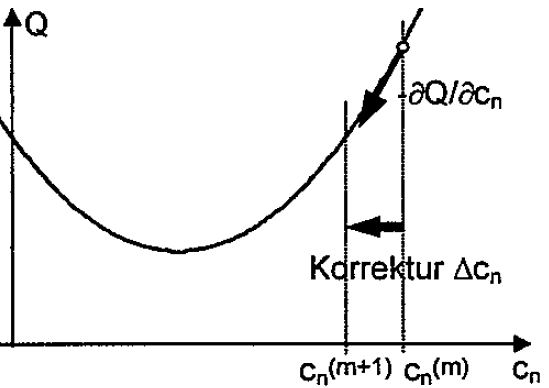
\includegraphics[width=\textwidth]{Content/AdaptSigVer/lmsAlgorithmus.png}
\end{minipage}
\textbf{Normalized Least Mean Square (NLMS):} $\qquad \qquad \qquad \qquad \alpha(i) = \frac{\alpha_0}{\delta + L \cdot \sigma^2} \qquad L=N+1$\\
$\delta$: kleiner Wert (verhindert Div durch 0); $\alpha_0$: Konstante;\\ 
Korrekturkonstante $\alpha$ umgekehrt proportional zur gesch�tzten Signalleistung $\sigma^2$\\
$\sigma^2$ wird als Kurzmittel der quadrierten Eingangssignalwerte $s^2(i)$ gebildet; sinnvolle Mittelungszeit $\rightarrow$ Filterl�nge $N+1$
